\documentclass{subfiles}

\begin{document}

	

\section{Introduction}

\par To briefly sum up the previous sections, FW LiDAR data (Section \ref{AcquireData}) are laser scanning data particularly useful in Forestry and inthis thesis they voxelised (Section \ref{Voxelisation}) using the open source software DASOS (Section \ref{DASOS}).  

\par This chapter focuses on constructing the surface of the scanned area from the voxelised FW LiDAR in 3D. On the one hand, the voxelised space can be directly rendered using ray-tracing \cite{Hanrahan1983}, but ray-tracing continouesly produces 2D images and even though near real time visualisation has been achieved ***cite ***, GPU processing and hyperformance computing is used. On the other hand, polygonisation (or isosurface extraction or surface reconstruction) it takes longer to generate but once generated it can be faster rendered using rasterisation. 

with commotity *** and the user can easily interact with the mesh in real time. For example, selecting a tree and measuring the distance between two locations, useful tasks in forestry. For that reason the polygonisation direction is taken.

\par The output is a 3D triangular polygon mesh. The standard rasterati

Find the surface of the Voxelised FW LiDAR and construct a polygon mesh, which is defined by vertices, edges and faces (triangles). 

Standard rendering format of GPUs 

Direct visualisation of volumetric data is also possible but more difficult to interact at real time 





\section{Algebraic Representation of the Volume}

Give a mathematical definition of the 

algebraic objects - implicit and functional are the same 

\par Algebraic objects were introduced by Blinn in 1982 \cite{Blinn1982} and enable the definition of complex objects without saving a large amount of triangles. Each one is defined by a function $ \mathit{f(X)} $ and the iso-surface value $\alpha$. The iso-surface value defines the boundaries of the object; for an object $ [f(x),a]$ every n-dimensional point $ \mathit{X} $  that lies on the surface of the object satisfies the condition $ \mathit{f(X)=\alpha }  $. To be more specific, all the following rules apply according to Pasko et al \cite{Pasko1994}: 
\begin{itemize}
	\item $	\mathrm{f(X) = \alpha }$ , when $X$ lies on the surface of the algebraic object
	\item $	\mathrm{f(X) > \alpha }$ , when $X$ lies inside the algebraic object and
	\item $	\mathrm{f(X) < \alpha }$ , when $X$ lies outside the algebraic object	 
\end{itemize}

\par Once the discrete density volume is generated, an algebraic object is defined to represent the scanned area. 

\par Regarding the algebraic representation of the 3D voxelised FW LiDAR data, X is a three dimensional point $\mathit{(x, y, z) }$ representing the longitude, latitude and height respectively and ${f(X)}$ is a function that takes  $\mathit{X}$ as input and returns the accumulated intensity value of the voxel that  $\mathit{X}$ lies inside. Also, the iso-surface value $\mathit{\alpha }$ is a user defined parameter and it is noise dependant (Please look at figure \ref{fig:SwitchingVisParameters} to understand how the iso-surface value affects the algebraic representation of voxelised FW LiDAR data). 




\section {Surface Reconstruction}\label{sec:SurfaceReconstruction}
\par Even though numerical implicitisation is beneficial in reducing storage memory and for various resolution renderings of the same object, visualising numerical/algebraic objects is not straight forward, since they contain no discrete values. This problem can either be address either by ray-tracing or polygonisation. In 1983, Hanraham suggested a ray-tracing approach, where an equation is derived from the ray and surface intersection \cite{Hanrahan1983}.  

\par The Marching Cubes algorithm was later introduced for polygonising implicit objects, using a look up table. Let’s assume that $f(X)$ defines an implicit object. At first the space is divided into cubes. Each cube is defined by eight corner points, which lie either inside or outside the object. By enumerating all the possible cases and linearly interpolating the intersections along the edges, the surface of the implicit object is constructed \cite{Lorensen1987}. According to Lorensen and Cline, the normal of each vertex is calculated by measuring the gradient change. But in this case, due to the high gradient changes inside the volume, this approach of calculating the normal leads to a non-smooth visualisation. For that reason, the normal of each vertex is derived by the average of its adjacent triangles. 

\par Further the sampling of the Marching cubes is independent from the sampling of the 3D density volume, but consistency between the two is required (Figure \ref{fig:MCSampling}). Let’s assume the discrete volume has (n * m * k) voxels. The volume can be sampled into cubes at any rate but to reduce artifacts a ((n+1) *(m+1) * (k+1)) dimensional sampling is suggested. Please note that every point that lies outside the volume is considered to be below the boundary threshold and set to a value lower than the isosurface value. An example of the corresponding sampling in 2D is shown on Figure 1, where the black grid represents a 2D density table and the blue grid represents the sampling used in during polygonisation.

\par The following Figura \ref{fig:SamplingArtifacts} shows the effects of oversampling during polygonisation. The right image was oversampled and the second one was sampled as explained above.

    %% Sampling
    \begin{figure} [h!]
    	\begin{subfigure}[t]{.49\textwidth}
    		
    		\centering
    		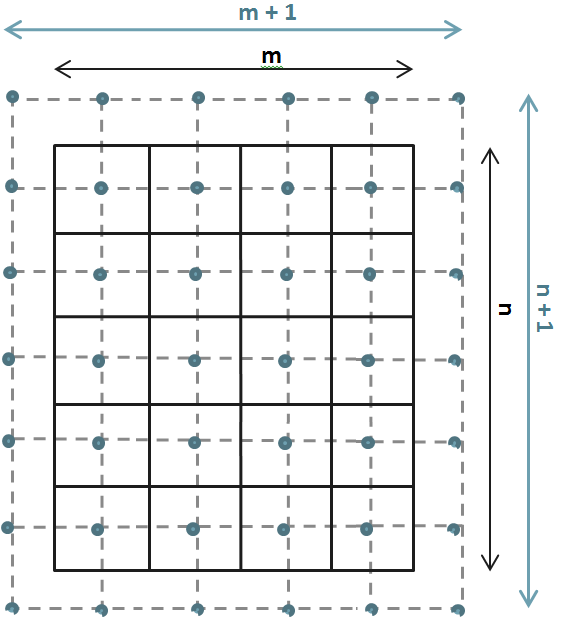
\includegraphics[width=.9\textwidth]{img/Sampling}
    		\caption{Suggested Sampling of the Marching Cubes Algorithm}
    		\label{fig:ExpectedSampling}
    	\end{subfigure} \hfill
    	\begin{subfigure}[t]{.49\textwidth}
    		\centering
    		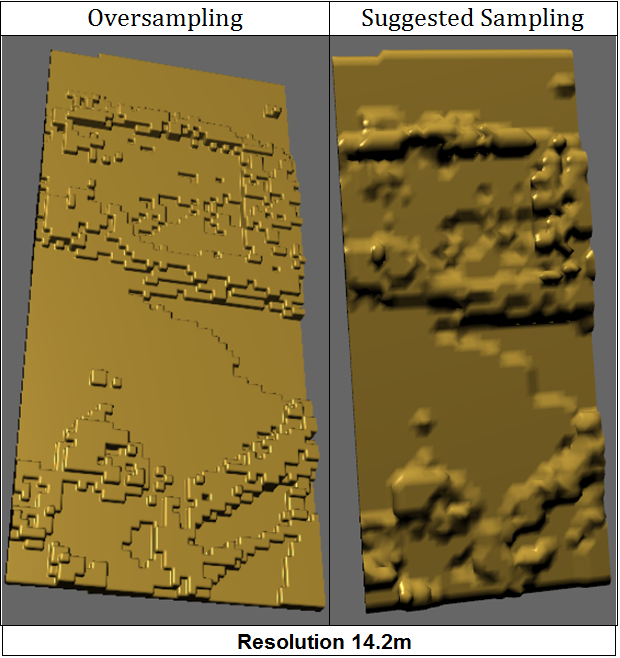
\includegraphics[width=.9\textwidth]{img/OversamplingVsSuggestedSampling}
    		\caption{Artifacts of Oversampling the Marching Cubes Algorithm} 
    		\label{fig:SamplingArtifacts}
    	\end{subfigure} \hfill
    	\caption{Marching Cubes Suggested Sampling}
    	\label{fig:MCSampling}
    \end{figure}


\subsection{Results}

 
 selecting region of interest \&
 

 \begin{figure} [h!]
 	\centering
 	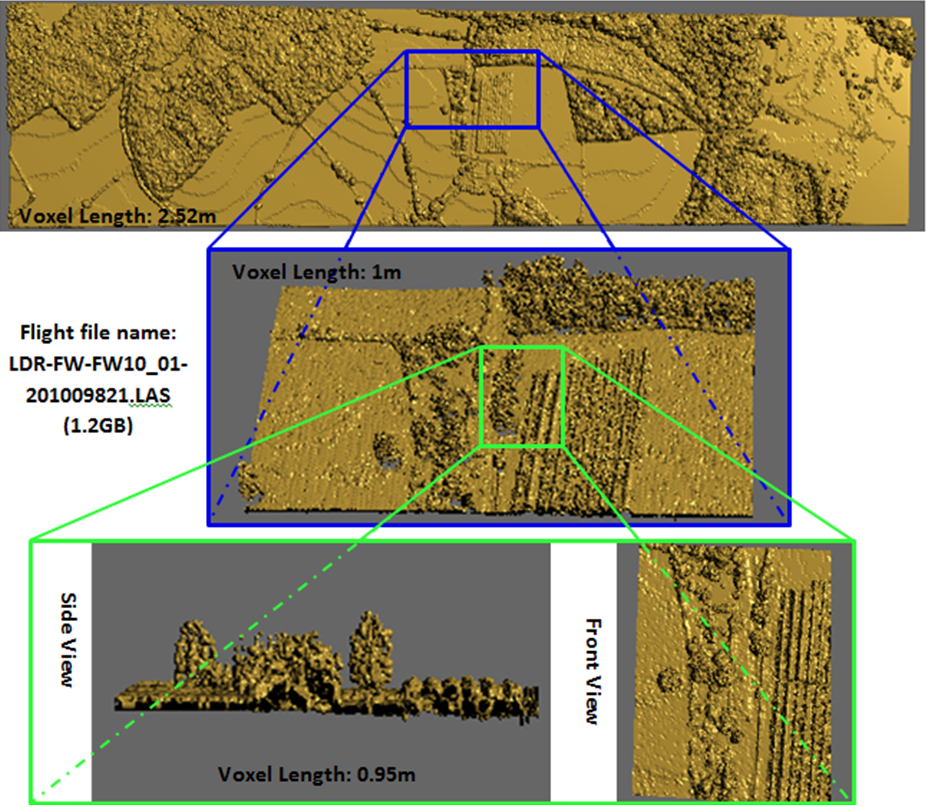
\includegraphics[width=.8\textwidth]{img/SelectingRegionOfInterest}
 	\caption[Selecting Region of Interest]{Selecting Region of Interest}
 	\label{fig:SelectingRegionOfInterest}
 \end{figure}
 
 
  \begin{figure} [h!]
  	\centering
  	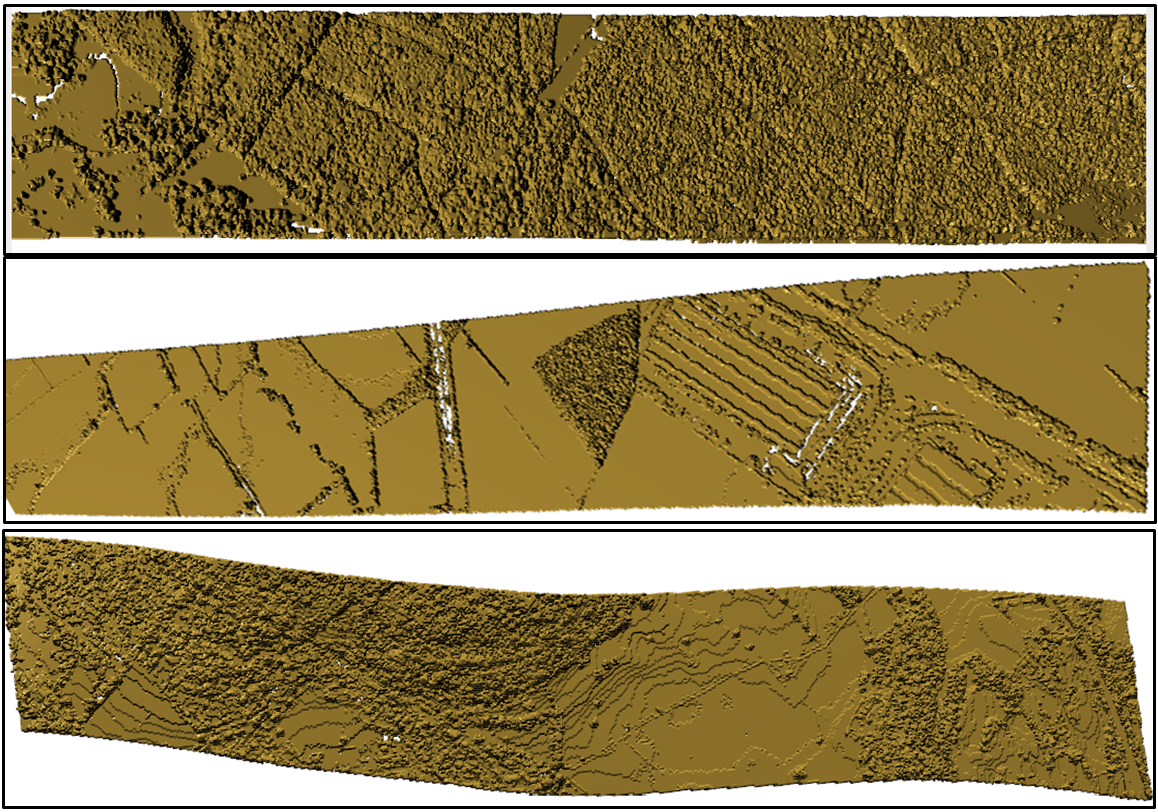
\includegraphics[width=.8\textwidth]{img/VariousFlightlines}
  	\caption[Various Flightlines Visualisation]{Polygonising NERC-ARF FW LiDAR data captured at different areas (New Forest, Milton Keynes and Eaves Wood)}
  	\label{fig:VariousFlightlines}
  \end{figure}
  

  
  \begin{figure} [h!]
  	\centering
  	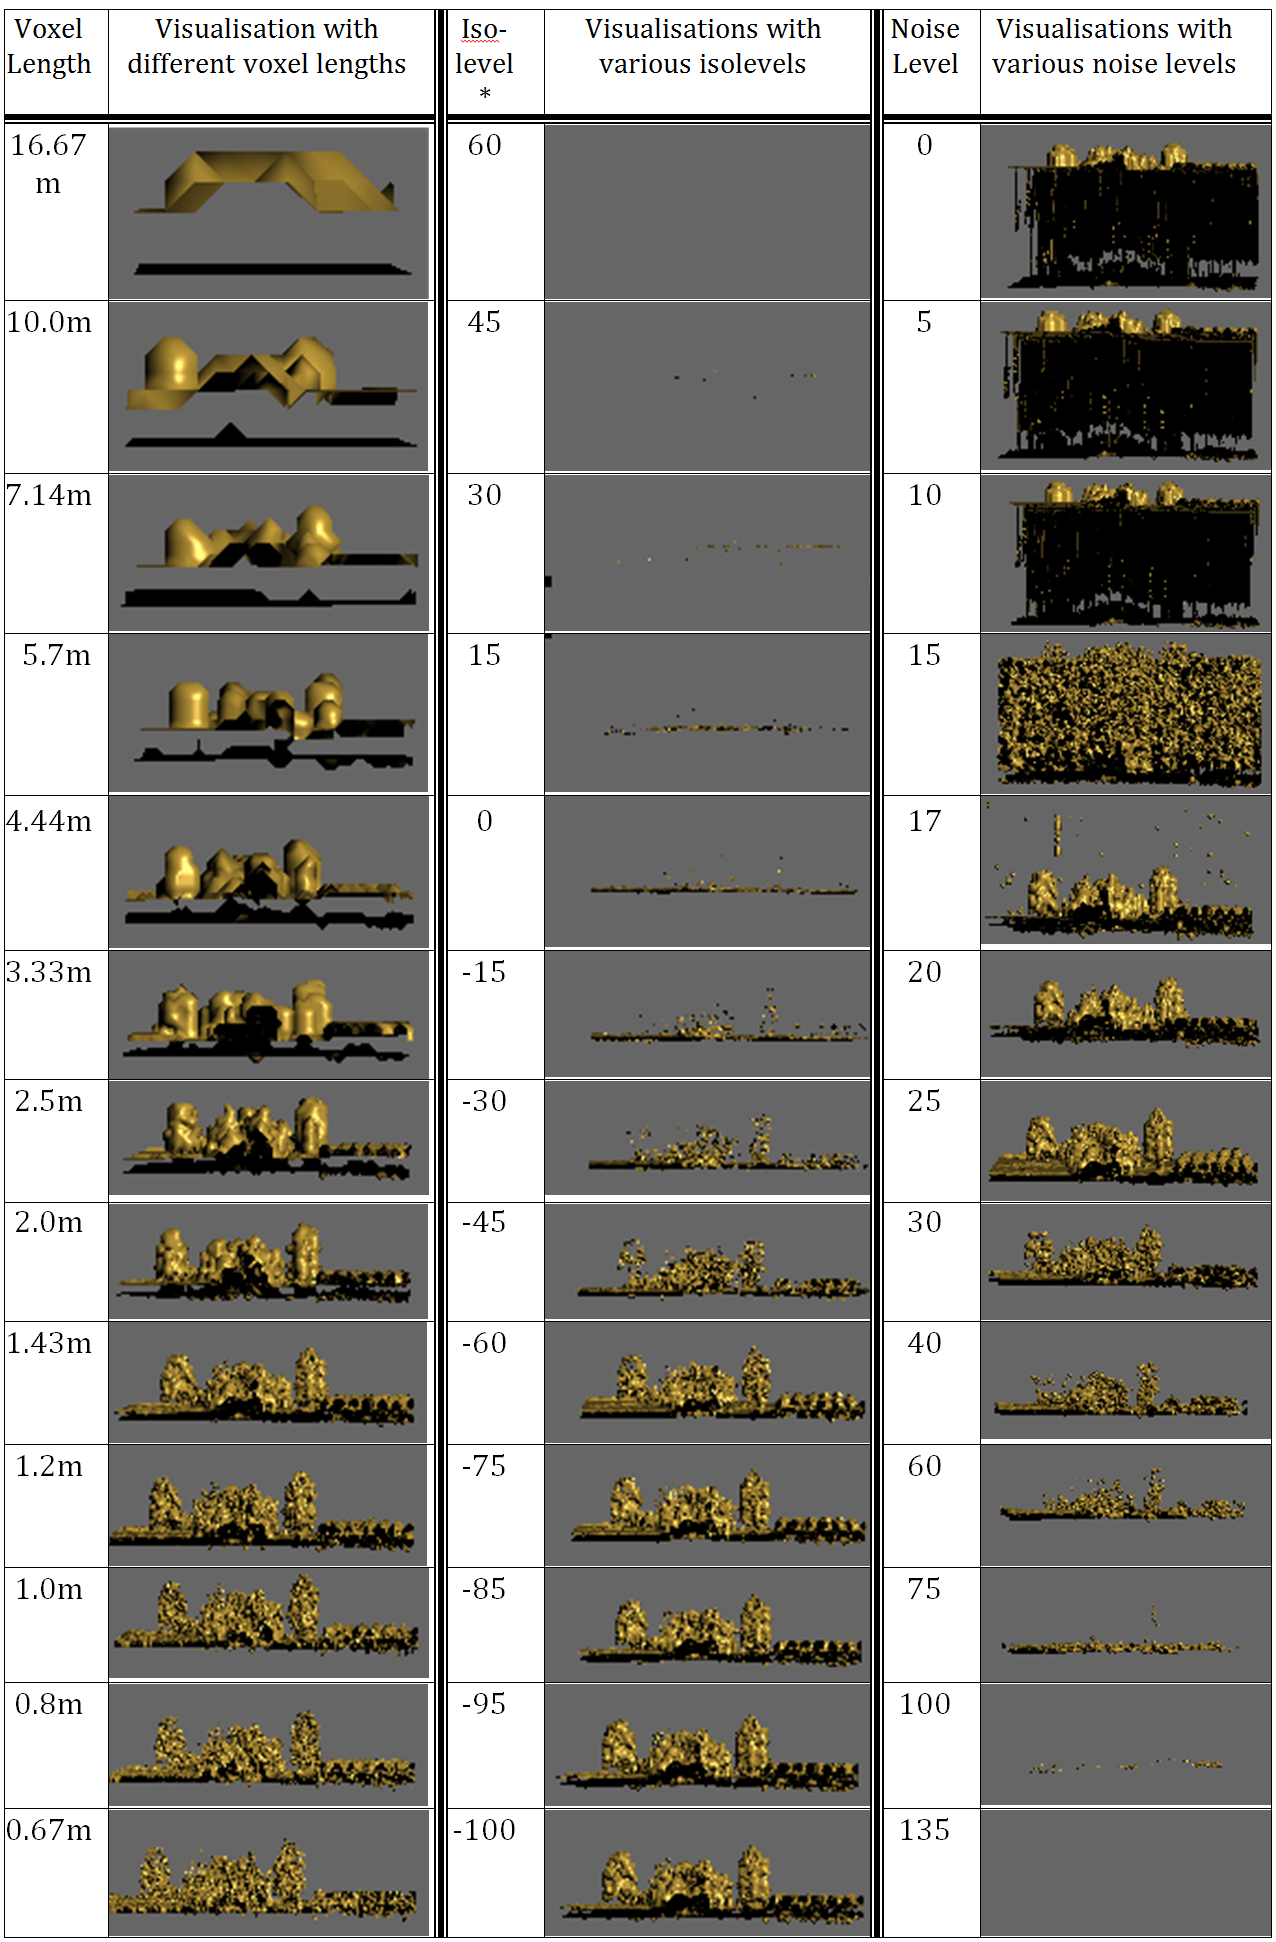
\includegraphics[width=0.95\textwidth]{img/SwitchingParameters}
  	\caption[Polygonisation Parameters]{How the output polygon mesh is affected by modifying the user-defined parameters}
  	\label{fig:SwitchingVisParameters}
  \end{figure}
  
   \begin{figure} [h!]
	   	\centering
    	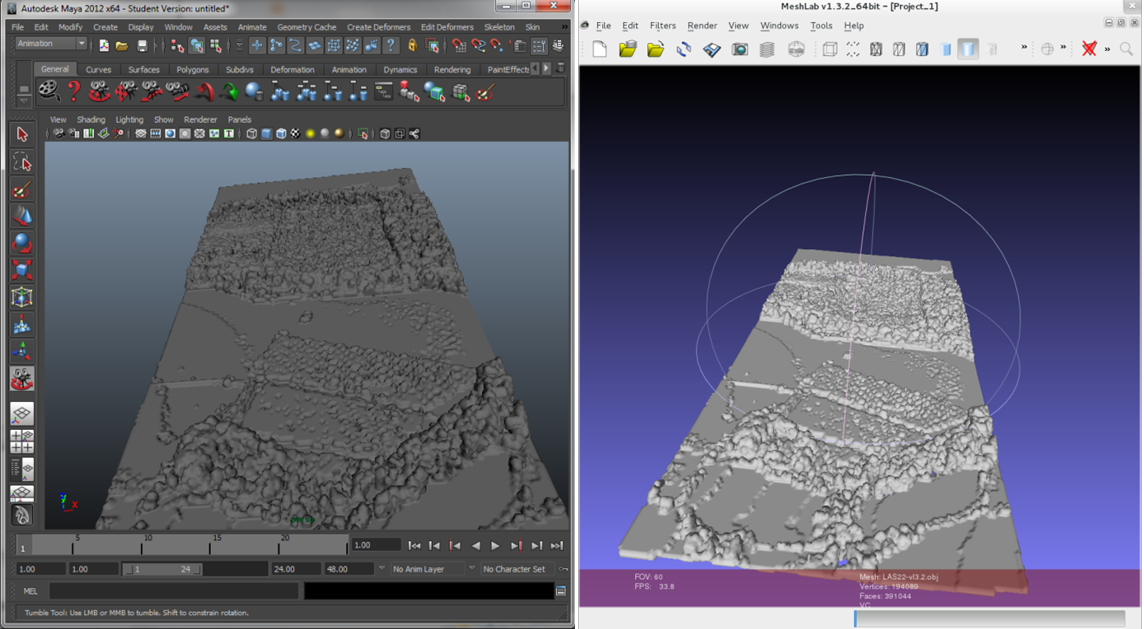
\includegraphics[width=0.9\textwidth]{img/AimationPackages.png}
     	\caption[Animation Packages]{Visualising the output of DASOS into animation software packages (Maya and Meshlab)}
     	\label{fig:AnimationPackages}
    \end{figure}
  
   \begin{figure} [h!]
   	\centering
   	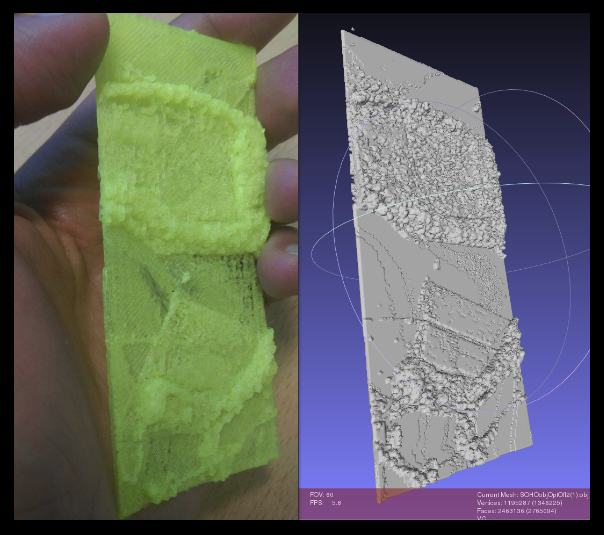
\includegraphics[width=0.9\textwidth]{img/NF-3Dprint}
   	\caption[3D printing]{3D printing of New Forest FW LiDAR data}
   	\label{fig:3Dprinting}
   \end{figure}

 

\end{document}